% MEGA extended abstract
%
%
%
%
%%%%%%%%%%%%%%%%%%%%%%%%%%%%%%%%%%%%%%%%%%%%%%%%%%%%%%%%%%%%%%%%%%%%%%%%%%%%%%%%%
\documentclass[12pt]{amsart}
\usepackage[margin = 1in]{geometry}
\usepackage{amsmath,amssymb,amsthm}
\usepackage[dvipsnames]{xcolor}
\usepackage{ulem}  % strike out text
\usepackage{graphicx}
\usepackage{tikz,verbatim}
%\pdfoutput=1

\usepackage{framed}

%Environments
\newtheorem{theorem}{Theorem}
\newtheorem{theorem'}{Theorem*}
\newtheorem{lemma}[theorem]{Lemma}
\newtheorem{corollary}[theorem]{Corollary}
\newtheorem{proposition}[theorem]{Proposition}
\newtheorem{algorithm}[theorem]{Algorithm}

\theoremstyle{definition}
\newtheorem{definition}[theorem]{Definition}
\newtheorem{example}[theorem]{Example}
\newtheorem{remark}[theorem]{Remark}


\title{Computing Galois Groups of Finite Fano Problems}
%%%%%%%%%%%%%%%%%%%%%%%%%%%%%%%%%%%%%%%%%%%%%%%%%%%%%%%%%%%%%%%%%%%%%%%%%%%% 
\author[T.~Yahl]{Thomas Yahl} 
\address{T.~Yahl\\ 
         Department of Mathematics\\ 
         Texas A\&M University\\ 
         College Station\\ 
         Texas \ 77843\\ 
         USA} 
\email{thomasjyahl@math.tamu.edu} 
\urladdr{http://www.math.tamu.edu/~thomasjyahl} 
%%%%%%%%%%%%%%%%%%%%%%%%%%%%%%%%%%%%%%%%%%%%%%%%%%%%%%%%%%%%%%%%%%%%%%%%%%%%%%%%%%

%Macros
\newcommand{\CC}{\mathbb{C}}
\newcommand{\RR}{\mathbb{R}}
\newcommand{\ZZ}{\mathbb{Z}}
\newcommand{\gr}{\mathbb{G}}
\newcommand{\gal}{\mathcal{G}}

\newcommand{\defcolor}[1]{{\color{RoyalBlue}#1}}
\newcommand{\demph}[1]{\defcolor{{\sl #1}}}

%%%%%%%%%%%%%
%%Beginning%%
%%%%%%%%%%%%%
\begin{document}

%%%%%%%%%%%%
%%Sections%%
%%%%%%%%%%%%
%
%1) Introduction
%   i) Jordan historical context
%   ii) Harris' result
%   iii) Hashimoto and Kadets paper
%
%2) Galois Groups of Branched Covers 
%
%3) Numerical Algebraic Geometry
%   i) Homotopy continuation
%   ii) Numerical certification
%
%4) Finite Fano Problems
%   i) Debarre and Manivel results
%   ii) Hashimoto and Kadets results
%
%5) Computational Methods
%   i) Monodromy loops
%   ii) Harris' method
%
%6) Results
%



%%%%%%%%%%%%
%%Abstract%%
%%%%%%%%%%%%
\begin{abstract}
The problem of enumerating linear spaces of a fixed dimension on a variety is known as a Fano problem. Those Fano problems with finitely many solutions have an associated Galois group that acts on the set of solutions. For a class of Fano problems, Hashimoto and Kadets determined the Galois group completely and showed that for all other Fano problems the Galois group contains the alternating group on its solutions. For Fano problems of moderate size with as yet undetermined Galois group, computational methods can be used to prove that the Galois group is the full symmetric group. For larger examples we give evidence the Galois group is the full symmetric group.
\end{abstract}
%%%%%%%%%%%%%%%%%%%%%%%%%%%%%%%%%%%%%%%%%%%%%%%%%%%%%%%%%%%%%%%%%%%%%%%%%%%%%%%%%

\maketitle

%%%%%%%%%%%%%%%%
%%Introduction%%
%%%%%%%%%%%%%%%%
\section{Introduction}
%Historical context of Fano problems
%   Debarre and Manivel
%
A Fano problem consists of computing or enumerating linear spaces of a specified dimension lying on a variety, such as the problem of 27 lines on a cubic surface. When the variety $X$ is a complete intersection, the set of linear spaces on $X$ was studied by Debarre and Manivel \cite{DM} in which they determined invariants such as its dimension and degree. We concern ourselves with only those Fano problems with a finite number of solutions, which we simply call a Fano problem. 

%Galois groups of fano problems (Jordan/Harris/Hashimoto & Kadets)
%   Jordan & Harris
%   Hashimoto & Kadets
%
%   We call a problem and its Galois group \defcolor{enriched} if the intrinsic structure restricts the Galois group from being the full symmetric group. If there are no obstructions and the Galois group is the full symmetric group, we call the problem and its Galois group \defcolor{fully symmetric}. 
%
To each Fano problem there is an associated Galois group. Jordan was the first to study these Galois groups in his work  ``Trait\'{e} des Substitutions et des \'{E}quations Alg\'{e}briques" in which he noted the Galois group of an enumerative problem must preserve any intrinsic structures of the problem \cite{Jordan}. The incidence structure of the lines on a cubic surface form a remarkable configuration, from which Jordan determined the Galois group is a subgroup of $E_6$. 

Harris progressed the study of Galois groups of Fano problems by proving Jordan's inclusion to be an equality and by showing that for $n\ge 4$ the Fano problems of lines in $\mathbb{P}^n$ on a hypersurface of degree $2n-3$, each of the Galois groups is the symmetric group on its solution set \cite{Harris}. Harris utilized that the algebraic Galois groups Jordan defined are geometric monodromy groups, an idea tracing back to Hermite \cite{Hermite}. After first showing these Galois groups are two-transitive, Harris showed each contains a simple transposition and therefore is the entire symmetric group. 

Much of the study of Galois groups of Fano problems then laid dormant until Hashimoto and Kadets nearly determined the Galois groups in all cases \cite{HK}. The Fano problems of $r$-planes in $\mathbb{P}^{2r+2}$ on the intersection of two quadrics were shown to have Galois group equal to the Weyl group $W(D_{2r+3})$ and all as yet undetermined Galois groups were shown to contain the alternating group on their solution set.

%Hashimoto and Kadets determined a class of Fano problems to be enriched and determined their Galois groups completely by a detailed study of the problems. They then determined that all other Galois groups must contain the alternating group on their solutions. This portion of their work also utilized showing that these Galois groups are highly transitive.

%This paper does computations
%   Methods
%   Results
%
By the results of Hashimoto and Kadets, a complete classification of the Galois groups of Fano problems rests on determining whether each of the remaining Galois groups is the alternating group or the symmetric group on its solutions. One way of making this distinction is to produce or show the existence of a simple transposition in the Galois group. For Fano problems of moderate size, this can be done computationally via methods of numerical homotopy continuation and numerical certification respectively.

Methods of numerical homotopy continuation can be used to simulate path liftings, which with a high degree of confidence produces permutations in the Galois group \cite{ngalois}. We do this and provide strong evidence for those Fano problems with up to $30,000$ solutions whose Galois group has yet to be determined that the Galois group is the entire symmetric group.

Harris' technique of showing a Galois group contains a simple transposition can be achieved with exact computations through numerical certification. For those Fano problems with up to $3,000$ solutions whose Galois group is yet to be determined, we use this to constitute a proof that the Galois group is the entire symmetric group. 



%%%%%%%%%%%%%%%%%%%%%%%%%%%%%%%%%%%%
%%Galois Groups of Branched Covers%%
%%%%%%%%%%%%%%%%%%%%%%%%%%%%%%%%%%%%
\section{Galois Groups of Branched Covers}
%Brached cover definition
%   varieties X,Y
%   branched cover \pi:X\to Y
%   degree d
%   
A map of algebraic varieties is dominant if the closure of its image is its target. A \defcolor{branched cover} is a dominant map $\pi:X\to Y$ of irreducible (complex) varieties of the same dimension. There is a maximal nonempty Zariski open set $U\subseteq Y$ (dense, open, and path-connected) such that for $y\in U$, the fiber $\pi^{-1}(y)$ has a fixed cardinality $d$ called the \defcolor{degree of $\pi$}. The complement $B = Y\setminus U$ is called the \defcolor{branch locus} of $\pi$.



%Galois groups definition
%   Galois group of pi $\gal_\pi$
%   Include image?
%
The restriction $\pi:\pi^{-1}(U)\to U$ is a covering space of degree $d$. Given a base point $y\in U$, each loop in $U$ based at $y$ lifts to $d$ paths in $\pi^{-1}(U)$ each starting at different points of the fiber $\pi^{-1}(y)$. The endpoints of these lifted paths give a permutation of the fiber $\pi^{-1}(y)$. The set $\gal_\pi$ of all permutations obtained in this way is the \defcolor{Galois} or \defcolor{monodromy group} of $\pi$. More detail about monodromy groups of covering spaces can be found in \cite{Hatcher}. 

Since $X$ is irreducible, $\pi^{-1}(U)$ is path-connected and so $\gal_\pi$ is transitive. Questions about higher transitivity can be reduced to irreducibility of certain fiber products \cite{ngalois,GGEGA}. A Galois group $\gal_\pi$ is \defcolor{enriched} if it is not the full symmetric group and otherwise we say the Galois group is \defcolor{fully symmetric}.



%Galois = monodromy
%
Historically, Jordan defined these Galois groups algebraically \cite{Jordan}. A branched cover $\pi:X\to Y$ induces an injection of function fields of these varieties $\mathbb{C}(Y)\hookrightarrow\mathbb{C}(X)$ so that $\mathbb{C}(X)$ is an algebraic extension of $\mathbb{C}(Y)$ of degree equal to the degree of $\pi$. The Galois group of $\pi$ is then defined as the Galois group of the extension $K/\mathbb{C}(Y)$, where $K$ is the Galois (normal) closure of $\mathbb{C}(X)$ over $\mathbb{C}(Y)$. The equivalence of the geometric definition with this algebraic definition was shown by Harris \cite{Harris}, but it goes back to Hermite. 

%While we won't make use of this algebraic definition, it allows for techniques of algebraic number theory to be used in studying Galois group in addition to the numerical methods we use. A method of Frobenius can be used to sample cycle types of elements of the Galois group as in \cite{GGEGA}. The Chebotarev density theorem shows that this sampling tends to uniformly sample cycle types of elements from the Galois group. {\color{red}(this isn't necessary2)}



%Numerical computation of Galois groups
%
Numerical algebraic geometry can be used to effectively compute Galois groups of branched covers as described in \cite{ngalois}. Given a branched cover $\pi:X\to Y$ and equations determining the varieties $X$ and $Y$, the paradigm of numerical homotopy continuation allows one to numerically lift paths from $Y$ to $X$. Lifting based loops in $Y$ then produces permutations belonging to the Galois group with a high degree of confidence. 

The technique of Harris showing the existence of a simple transposition in the Galois group relies on showing that a fiber $\pi^{-1}(y)$ contains a single point of multiplicity 2. Smale's alpha theory permits methods of numerical certification to verify the existence of such a fiber and simple transposition.



%%%%%%%%%%%%%%%%%%%%%%%%
%%Finite Fano Problems%%
%%%%%%%%%%%%%%%%%%%%%%%%
\section{Finite Fano Problems}
%Definitions
%   Historical context?
%
The family of $r$-planes in $\mathbb{P}^n$ is an irreducible projective variety known as the \defcolor{Grassmanian variety} $\gr(r,n)$. For a variety $X\subseteq\mathbb{P}^n$ its \defcolor{Fano scheme} is the subscheme of $\gr(r,n)$ of $r$-planes that lie on $X$. 

When the variety $X$ is a complete intersection, the Fano scheme is classified by the finite data of the dimension $r$ of the linear spaces, the dimension $n$ of the ambient projective space, and the weakly-increasing sequence of degrees $d_\bullet = (d_1,\dotsc,d_s)$ (with $d_1>1$) of the polynomials defining the variety $X$. We write this data as a tuple $(r,n,d_\bullet)$.

Let $\mathbb{C}^{(r,n,d_\bullet)}$ denote the parameter space of systems of homogeneous polynomials $F = (f_1,\dotsc,f_s)$ in $n+1$ variables of respective degrees $d_\bullet = (d_1,\dotsc,d_s)$. For generic $F\in\mathbb{C}^{(r,n,d_\bullet)}$ the zero set $X = \mathcal{V}(F)$ defines a complete intersection of dimension $n-s$ for which we would like to describe the Fano scheme of $r$-planes. When $n-s<2r$ there are no $r$-planes on $X$, so we require that $n-s\ge 2r$. We write $\mathcal{V}_r(F)$ for this Fano scheme.



%Dimension & degree
%
Fix a system $F=(f_1,\dotsc,f_s)\in\mathbb{C}^{(r,n,d_\bullet)}$. The condition that the homogeneous polynomial $f_i$ vanishes along an $r$-plane $\ell\in\gr(r,n)$ amounts to the vanishing of the $\left(\begin{smallmatrix}r+d_i\\d_i\end{smallmatrix}\right)$ coefficients that arise when writing $f_i$ in local coordinates on $\ell$. Since the Grassmanian $\gr(r,n)$ has dimension $(r+1)(n-r)$, the expected dimension of the Fano scheme $\mathcal{V}_r(F)$ is given by
\begin{align*}
\delta(r,n,d_\bullet) = (r+1)(n-r) - \sum_{i=1}^s\begin{pmatrix}r+d_i\\d_i\end{pmatrix}.
\end{align*}
Debarre and Manivel \cite{DM} showed that when $\delta(r,n,d_\bullet)\ge 0$, the Fano scheme of a general $F\in\mathbb{C}^{(r,n,d_\bullet)}$ is reduced and of the expected dimension $\dim\mathcal{V}_r(F) = \delta(r,n,d_\bullet)$. When $\delta(r,n,d_\bullet)<0$ the Fano scheme $\mathcal{V}_r(F)$ is empty for general $F\in\mathbb{C}^{(r,n,d_\bullet)}$. 

%Debarre and Manivel showed that when $\delta(r,n,d_\bullet)\ge 0$, there is a Zariski open set $U_{(r,n,d_\bullet)}\subseteq\mathbb{C}^{(r,n,d_\bullet)}$ so that for $F\in U_{(r,n,d_\bullet)}$, the Fano scheme has the expected dimension $\dim\mathcal{V}_r(F) = \delta(r,n,d_\bullet)$ \cite{DM}. When $\delta(r,n,d_\bullet)<0$, the Fano scheme is generically empty. 

We concern ourselves with those Fano schemes which are zero-dimensional. We say a \defcolor{Fano problem} is the problem of describing those Fano schemes $\mathcal{V}_r(F)$ determined by general homogeneous polynomials $F\in \mathbb{C}^{(r,n,d_\bullet)}$ when $\delta(r,n,d_\bullet) = 0$.

Since the Grassmanian is a projective variety, a Fano scheme $\mathcal{V}_r(F)$ has a well-defined degree. For Fano schemes determined by generic $F\in\mathbb{C}^{(r,n,d_\bullet)}$, this degree has been determined by techniques from intersection theory and can be written explicitly. 

Define the quantities
\begin{align*}
Q_{r,d}(x) = \prod_{a_0+\dotsb+a_r=d}(a_0x_0 + \dotsb + a_rx_r)\in\mathbb{Z}[x_0,\dotsb,x_r],~a_i\in\mathbb{Z}_{\ge 0}
\end{align*}
and $Q_{r,d_\bullet}(x) = Q_{r,d_0}(x)\dotsb Q_{r,d_s}(x)$, as well as the Vandermonde polynomial
\begin{align*}
V_r(x) = \prod_{0\le i<j\le r}(x_i-x_j).
\end{align*}
When $\delta(r,n,d_\bullet) = 0$, the degree $\text{deg}(r,n,d_\bullet)$ of a Fano scheme $\mathcal{V}_r(F)$ determined by general polynomials $F\in \mathbb{C}^{(r,n,d_\bullet)}$ is equal to the coefficient of $x_0^n x_1^{n-1}\dotsb x_r^{n-r}$ in the product $Q_{r,d_\bullet}(x)V_r(x)$ \cite{DM}. Table \ref{Small Fano} shows the degrees of Fano problems with a small number of solutions.
\begin{table}[htb]
  \caption{Small Fano problems}
  \label{Small Fano}
  \def\arraystretch{1.2}
  \begin{tabular}{||c|c|c|c|c||}
    \hline
    $r$ & $n$ & $d_\bullet$ & $\#$ of solutions & Galois Group\\
    \hline\hline
    1 & 4 & $(2,2)$ & 16 & $D_5$\\
    \hline
    1 & 3 & $(3)$ & 27 & $E_6$\\
    \hline
    2 & 6 & $(2,2)$ & 64 & $D_7$\\
    \hline
    3 & 8 & $(2,2)$ & 256 & $D_9$\\
    \hline
    1 & 7 & $(2,2,2,2)$ & 512 & $S_{512}$\\
    \hline
    1 & 6 & $(2,2,3)$ & 720  & $S_{720}$\\
    \hline
    4 & 10 & $(2,2)$ & 1024 & $D_{11}$\\
    \hline
    2 & 8 & $(2,2,2)$ & 1024  & $S_{1024}$\\
    \hline
    1 & 5 & $(3,3)$ & 1053  & $S_{1053}$\\
    \hline
    1 & 5 & $(2,4)$ & 1280  & $S_{1280}$\\
    \hline
    1 & 4 & $(5)$ & 2875 & $S_{2875}$\\
    \hline
  \end{tabular}
\end{table}



%Galois groups of Fano problems
%
The data $(r,n,d_\bullet)$ of a Fano problem determines an incidence correspondence.
\begin{center}
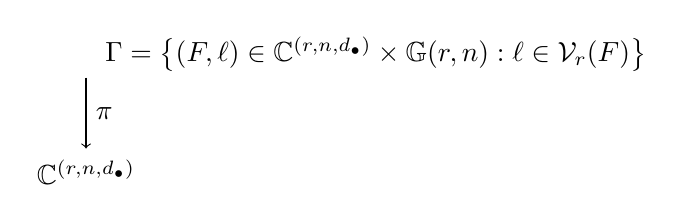
\begin{tikzpicture}
\node at (0,1.5) {$\Gamma = \left\{ (F,\ell)\in\mathbb{C}^{(r,n,d_\bullet)}\times\gr(r,n):\ell\in\mathcal{V}_r(F) \right\}$};
\draw[->] (-3.68,1.2)--(-3.68,.3) node [right] at (-3.68,.75) {$\pi$};
\node at (-3.68,0) {$\mathbb{C}^{(r,n,d_\bullet)}$};
\end{tikzpicture}
\end{center}
By the results of Debarre and Manivel, there is a Zariski open set $U_{(r,n,d_\bullet)}$ with the property that if $F\in U_{(r,n,d_\bullet)}$, $\mathcal{V}_r(F)$ consists of $\deg(r,n,d_\bullet)$ smooth points. The restriction of $\pi$ to $\pi^{-1}(U_{(r,n,d_\bullet)})$ is then a covering space of degree $\text{deg}(r,n,d_\bullet)$ and so $\pi$ is a branched cover. We define the \defcolor{Galois group} of the Fano problem corresponding to the data $(r,n,d_\bullet)$ to be $\gal_{(r,n,d_\bullet)} = \gal_\pi$. 

These Galois groups were first studied by Jordan, who showed that $\gal_{(1,3,(3))}\subseteq E_6$ by studying the incidence structure of the 27 lines on a smooth cubic surface \cite{Jordan}. Harris later proved Jordan's inclusion to be an equality, $\gal_{(1,3,(3))}= E_6$, and studied a generalization of this problem. Harris showed that for $n\ge 4$, the Fano problem of lines in $\mathbb{P}^n$ on a hypersurface of degree $2n-3$ is fully symmetric \cite{Harris}.

Hashimoto and Kadets later took up the study of these Galois groups more generally. They studied the Fano problems of $r$-planes in $\mathbb{P}^{2r+2}$ on the intersection of two quadrics in great detail to determine $\gal_{(r,2r+2,(2,2))}=W(D_{2r+3})$. Hashimoto and Kadets then showed that if $(r,n,d_\bullet)$ is not the Fano problem $(1,3,(3))$ and $d_\bullet\ne(2,2)$, then $\gal_{(r,n,d_\bullet)}$ contains the alternating group on its solutions \cite{HK}.

We use techniques from numerical algebraic geometry to prove that for the remaining Fano problems with a moderate number of solutions, the Galois group is the full symmetric group. For those with more solutions, we provide strong evidence the Galois group is fully symmetric. 



%%%%%%%%%%%%%%%%%%%%%%%%%%%%%%%%
%%Numerical Algebraic Geometry%%
%%%%%%%%%%%%%%%%%%%%%%%%%%%%%%%%
\section{Numerical Algebraic Geometry}
%Numerical homotopy continuation
%   Citations?
%   Include image?
%
Let $P$ be a family of square systems of $m$ polynomials in $m$ variables such that a general system $E\in P$ has a finite \defcolor{solution set} $\mathcal{V}(E)$. A \defcolor{start system} $G\in P$ is a system with the maximal number of smooth solutions called \defcolor{start solutions}, each of which is already known and computed to some desired accuracy. Given a \defcolor{target system} $E\in P$ with unknown \defcolor{target solutions}, a \defcolor{homotopy} from $G$ to $E$ is a path $\mathcal{H}(x;t)\in P$ in the parameter space depending on a new parameter $t\in\mathbb{C}_t$ such that $\mathcal{H}(x;0) = G(x)$ and $\mathcal{H}(x;1)=E(x)$. The zero set $\mathcal{V}(\mathcal{H}(x;t))\subseteq\mathbb{C}^m\times\mathbb{C}_t$ projects dominantly to $\mathbb{C}_t$ and for $t_0\in\mathbb{C}_t$ the fiber over $t_0$ is the solution set $\mathcal{V}(\mathcal{H}(x;t_0))$. 

Since $G$ has the maximal number of smooth solutions, $\mathcal{V}(\mathcal{H}(x;t))$ contains a union of curves connecting start solutions to the isolated solutions of the target system \cite{Morgan}. Over a real path $\gamma\in\mathbb{C}_t$ from 0 to 1 avoiding any singular systems, these curves are solutions to initial-value problems starting at the start solutions. Repeatedly approximating solutions to the initial-value problems on small intervals and applying Newton's method leads to a ``predictor-corrector" method of approximating values along the curves. When the target solutions are smooth, predictor-corrector methods successfully approximate these solutions and if there are singular target solutions endgames readily approximate the solutions.

Numerical homotopy algorithms with these capabilities and more have been implemented in several software packages such as \texttt{Bertini} \cite{Bertini}, \texttt{NAG4M2} \cite{NAG4M2}, \texttt{HomotopyContinuation.jl} \cite{HCJL}, and \texttt{PHC} \cite{PHCpack}.



%Numerical certification
%
Once solutions to a system $E$ have been approximated, one would like some guarantee that the approximations actually lie near solutions or to refine the approximations further. Newton's method allows one to refine solutions, but there is no immediate guarantee that Newton's method will converge or if it converges, to the solution it is approximating. Smale's alpha theory sets a framework for making such guarantees for Newton's method. 

Given a polynomial system $E$ of $m$ polynomials in $m$ variables, we write
\begin{align*}
N_{E}(x) = \begin{cases} x - (DE(x))^{-1}E(x)~\text{ if }~DE(x)~\text{ is invertible} \\
x~\text{ otherwise}
\end{cases}
\end{align*}
for the \defcolor{Newton operator} of $E$ and $N_{E}^k(x)$ for its $k$-th iterate. A point $x\in\mathbb{C}^m$ is an \defcolor{approximate solution} of $E$ with \defcolor{associated solution} $\zeta\in\mathcal{V}(E)$ if for all $k\in\mathbb{N}$
\begin{align*}
||N_{E}^k(x) - \zeta||\le \left(\frac{1}{2}\right)^{2^k - 1}||x-\zeta||,
\end{align*}
where here $||\cdot||$ denotes the usual Euclidean norm on $\mathbb{C}^m$. 

To a square system $E$ and a point $x\in\mathbb{C}^m$, Smale defined the quantities $\alpha(E,x)$, $\beta(E,x)$, and $\gamma(E,x)$. The first quantity is the product $\alpha(E,x) = \beta(E,x)\gamma(E,x)$, where $\beta(E,x)$ is the size of a Newton step and $\gamma(E,x)$ is related to the derivatives of $E$. These quantities can determine whether a point $x\in\mathbb{C}^m$ is an associated solution to $E$ as follows.
%cite?
\begin{theorem}
If $E$ is a square system of equations in $m$ variables and $x\in\mathbb{C}^m$ is such that
\begin{align*}
\alpha(E,x) < \frac{13-3\sqrt{17}}{4} \approx .15767,
\end{align*}
then $x$ is an approximate solution of $E$. If $\zeta\in\mathcal{V}(E)$ is the associated solution to $x$, then $||x-\zeta||<2\beta(E,x)$. 
\end{theorem}
When the coefficients of $E$ and coordinates of $x$ are exact and the condition above can be verified, we say the approximate solution $x$ has been \defcolor{hard-certified}. This can be achieved when $E$ and $x$ have exact coefficients and coordinates in the Gaussian rationals $\mathbb{Q}(i)$. Numerical software such as \texttt{alphaCertified} \cite{alphaCertified} allows for the input system and solutions with Gaussian rational coefficients and coordinates for this reason.

When the hypotheses of the theorem are satisfied, we have that $x$ is an approximate solution to $E$ so that Newton's method converges rapidly and we have a bounding ball for the actual solution $\zeta$. We make use of this by showing the existence of distinct solutions to systems $E$ by using approximate solutions to provide distinct bounding balls for solutions of $E$. Since our approximate solutions are hard-certified, this constitutes a proof that there are distinct solutions for each of our approximate solutions.



%%%%%%%%%%%%%%%%%%%%%%%%%
%%Computational Methods%%
%%%%%%%%%%%%%%%%%%%%%%%%%
\section{Computational Methods and Results}
%Monodromy loops
%
Given data $(r,n,d_\bullet)$ for a Fano problem the Galois group $\gal_{(r,n,d_\bullet)}$ is the Galois group of the branched cover $\pi:\Gamma\to\mathbb{C}^{(r,n,d_\bullet)}$, defined by lifting paths from the base $U_{(r,n,d_\bullet)}$ to $\Gamma$. Given $F\in\mathbb{C}^{(r,n,d_\bullet)}$, the fiber $\pi^{-1}(F)$ is the Fano scheme $\mathcal{V}_r(F)$ which can be explicitly described by a set of equations $E$ in local coordinates on the Grassmanian $\gr(r,n)$. For $F\in U_{(r,n,d_\bullet)}$ these equations have $\text{deg}(r,n,d_\bullet)$ many smooth solutions, which can be computed to any desired accuracy by external software. 

Choose a base point $F\in U_{(r,n,d_\bullet)}$ so that the corresponding system $E$ in local coordinates on the Grassmanian $\gr(r,n)$ has $\text{deg}(r,n,d_\bullet)$ smooth solutions. A loop in $U_{(r,n,d_\bullet)}$ based at $F$ avoiding any singular Fano schemes $\mathcal{V}_r(F)$ gives a homotopy of the system $E$ with itself. With high confidence, tracking solutions of $E$ along this loop with numerical software yields the same permutation in the Galois group $\mathcal{G}_{(r,n,d_\bullet)}$ as obtained by lifting this loop.

By a theorem of Zariski, the Galois group of a branched cover is generated by lifting loops around components of the branch locus $B$. While components of the branch locus may be difficult to compute, individual points of $B$ may be found via heuristics. For those Fano problems of moderate size whose Galois group is undetermined, one can produce a simple transposition by lifting loops around a point in the branch locus. 

For those Fano problems with up to $30,000$ solutions and undetermined Galois group, a point in the branch locus $B$ was found and a base point $F\in U_{(r,n,d_\bullet)}$ was chosen nearby. Solutions to the equations $E$ describing the Fano scheme $\mathcal{V}_r(F)$ were found using techniques from \cite{monodromySolve} in \texttt{Macaulay2} \cite{M2}. These solutions were tracked around a small triangular path encircling the chosen point in the base locus using \texttt{NAG4M2} \cite{NAG4M2}. Since each of these Galois groups are either the alternating group or the symmetric groups, we obtain the following computational result.

\begin{theorem'}
With a high degree of confidence the Galois groups $\gal_{(1,7,(2,2,2,2))}$, $\gal_{(1,6,(2,2,3))}$, $\gal_{(2,8,(2,2,2))}$, $\gal_{(1,5,(3,3))}$, $\gal_{(1,5,(2,4))}$, $\gal_{(1,4,(5))}$, $\gal_{(1,10,(2,2,2,2,2,2))}$, and $\gal_{(1,9,(2,2,2,2,3))}$ are fully symmetric.
\end{theorem'}

The computations demonstrating this result can be replicated from the data in the \\
\texttt{MonodromyData} folder of the repository \cite{GithubRepo}. For each of the listed Fano problems there is a folder containing 2 files. In each folder, the file \texttt{baseData.txt} contains the data of a base point $F\in U_{(r,n,d_\bullet)}$, the corresponding system of equations $E$, and solutions to $E$. The file \texttt{loopData.txt} then contains points in $U_{(r,n,d_\bullet)}$ which trace out a trianglar loop encircling a point in the base locus $B$. The repository provided file \texttt{FanoProblems.m2} then uses \texttt{NAG4M2} to track these solutions along this loop and output the corresponding permutation.



%Harris' method
%
While these numerical liftings do not constitute a proof, they do provide strong evidence that these Galois groups are the full symmetric group in each case. To provide a proof of this result in some cases, we use a method of Harris. To show that the problem of lines in $\mathbb{P}^n$ on a hypersurface of degree $2n-3$ contains a simple transposition and is fully symmetric, Harris produced an $F\in \mathbb{C}^{(1,n,(2n-3))}$ with the property that the corresponding system $E$ has a unique multiple root of multiplicity 2. A small loop around $F$ then lifts to a simple transposition.

For $F\in \mathbb{C}^{(r,n,d_\bullet)}$, the system $E$ whose solutions describe the Fano scheme $\mathcal{V}_r(F)$ has at most $\text{deg}(r,n,d_\bullet)$ isolated solutions by the results of Debarre and Manivel. If the system $E$ has a multiple solution, it has a unique multiple solution of multiplicity 2 if there are exactly $\text{deg}(r,n,d_\bullet)-1$ distinct solutions. We use numerical certification to verify chosen systems have this property and hence prove the existence of a simple transposition in the Galois group for some Fano problems.

For those Fano problems with up to $20,000$ solutions and undetermined Galois group the following was achieved. First a linear space $\ell\in\gr(r,n)$ with Gaussian rational local coordinates in the Grassmanian was chosen. Then a system $F\in \mathbb{C}^{(r,n,d_\bullet)}$ with exact Gaussian rational coefficients was found with the property that the corresponding system of equations $E$ in local coordinates on the Grassmanian has a unique multiple root of multiplicty 2 corresponding to $\ell$. Every solution to $E$ was approximated by Gaussian rational points and hard-certified to be correspond to a distinct solution by \texttt{alphaCertified}, proving the claim. 

\begin{theorem}
The Galois groups $\gal_{(1,7,(2,2,2,2))}$, $\gal_{(1,6,(2,2,3))}$, $\gal_{(2,8,(2,2,2))}$, $\gal_{(1,5,(3,3))}$, $\gal_{(1,5,(2,4))}$, and $\gal_{(1,4,(5))}$ are fully symmetric.
\end{theorem}

The \texttt{CertificationData} folder of the repository \cite{GithubRepo} includes the data used to verify the claim above. For each of the listed Fano problems, there is a folder containing 2 files. The file \texttt{FanoData.txt} contains the data of the systems $F\in\mathbb{C}^{(r,n,d_\bullet)}$ and $E$ and the linear space $\ell$. The file \texttt{solutionData.txt} contains $\text{deg}(r,n,d_\bullet)-1$ approximate solutions to $E$ given with Gaussian rational coordinates. The repository provided file \texttt{FanoProblems.m2} uses \texttt{alphaCertified} to hard-certify each given solution corresponds to a distinct solution, proving the result.



\bibliographystyle{abbrv}
\bibliography{MEGA_Abstract}

\end{document}

%PROBLEMS?
%1) How do we know our system lies in U_(r,n,d_\bullet)?
%2) Make sure no computed solutions are singSoln or are too close to singSoln. (something something certification gives you unique solution in ball if alpha small enough?)
